\section{Introduction: Covering spaces}
A continuous map between spaces $p: Y \rightarrow X$ is a \emph{cover} or a \emph{covering map} if every point $x \in X$ has an open neighborhood $U$ such that \begin{enumerate}
  \item $p^{-1}(U)$ is a disjoint union of open sets $\sqcup_{i \in \cali} U_i$,
  \item $p$ restricted to each $U_i$ is an isomorphism.
\end{enumerate}
% \footnote{We'll later on show that the size of fiber does not depend on the point $x$.}
\begin{figure}[H]
  \centering
  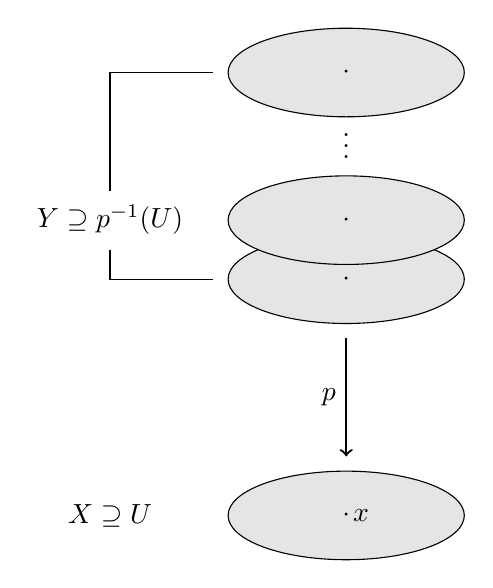
\begin{tikzpicture}[scale=0.75]
   \draw [black,fill=gray!20] (0,0)  ellipse (2cm and 0.75cm);
   \draw [black,fill=gray!20] (0,1) ellipse (2cm and 0.75cm);
   \draw [black,fill=gray!20] (0,3.5) ellipse (2cm and 0.75cm);
    \node at (0,2.4) {$\vdots$};
   \node at (0, 0) {$\boldsymbol{\cdot}$};
   \node at (0, 1) {$\boldsymbol{\cdot}$};
   \node at (0, 3.5) {$\boldsymbol{\cdot}$};
   \draw (-4,0.5) -- (-4,0) -- (-2.25,0);
   \draw (-4,1.5) -- (-4,3.5) -- (-2.25,3.5);
   \node at (-4, 1) {$Y \supseteq p^{-1}(U)$};

   \draw [thick,->] (0,-1) -- (0,-3) node[midway,left] {$p$};

   \draw [black,fill=gray!20] (0,-4)
      ellipse (2cm and 0.75cm);
   \node at (-4, -4) {$X \supseteq U$};
   \node at (0, -4) {$\boldsymbol{\cdot}$};
   \node at (0.25, -4) {$x$};

\end{tikzpicture}

  \caption{Pancake picture of covering spaces}
\end{figure}
$U$ is said to be an \emph{evenly covered neighborhood}.
If $\abs{p^{-1}(x)} = k$ for ever $x \in X$, we say that $p$ is a $k$-cover.

\begin{ex}
  The most basic example of a covering space is
  \begin{equation*}
    I \rightarrow \{*\}
  \end{equation*}
  where $I$ is a discrete set.
  This is not very interesting, so from now on \textbf{we will assume that all our spaces connected.}
\end{ex}

\begin{ex}
  The only connected cover of $[0,1]$ is the space $[0,1]$ inself.
\end{ex}

\begin{ex}
  The first non-trivial example of a cover comes from a circle.
  \begin{align*}
    S^1 &\longrightarrow S^1 \\
    \theta \mod 2 \pi &\longmapsto n \theta \mod 2\pi
  \end{align*}
  The real line is also a cover of $S^1$.
  \begin{align*}
    \bbr^1 &\longrightarrow S^1 \\
    \theta &\longmapsto \theta \mod 2\pi
  \end{align*}
\end{ex}

\begin{ex}
  Turns out, the cylinder is a 2-covering of a mobius strip.
  It is hard to describe this using coordinates or equations, we'll instead do this combinatorially.
\end{ex}






\subsection{Spaces}
We will use cell complexes as a combinatorial model for spaces.
A \emph{2-cell complex} $X$ is a triple $(V, E, F)$ consisting of:
  \begin{enumerate}
    \item A non-empty set of vertices $V$.
    \item A set of directed edges $E$. For each edge $e \in E$, denote by $d_0 e$ and $d_1 e$ the starting and ending vertex of $e$ respectively. Denote by $e^{-1}$ the same edge but going in the opposite direction so that $d_0 e^{-1} = d_1 e$ and $d_1 e^{-1} = d_0 e$.
    \item A set of faces $F$.
  \end{enumerate}
  We further assume that our cell complexes are
  \begin{enumerate}
    \item \emph{locally finite} i.e. there are finitely many edges between any two vertices, and
    \item \emph{connected} i.e. there is a path of undirected edges connecting any two vertices.
  \end{enumerate}

A \emph{simplical map} between two cell complexes $p: X_0 \rightarrow X_1$ is a compatible triple of maps.
\begin{align*}
  V_0 \rightarrow V_1 && E_0 \rightarrow E_1 && F_0 \rightarrow F_1
\end{align*}
A simplical map is a covering space map if the induced map on the underlying topological spaces is one.

\begin{remark}
  Not every continuous map can be represented by a simplicial map, but every covering map can be. Further, there are more than one ways to describe a space using a graph.
\end{remark}






\subsubsection{Example: Covers of $S^1$}
For every integer $n$, there exists a unique $n$-cover of a circle.
  \begin{figure}[H]
  \centering
    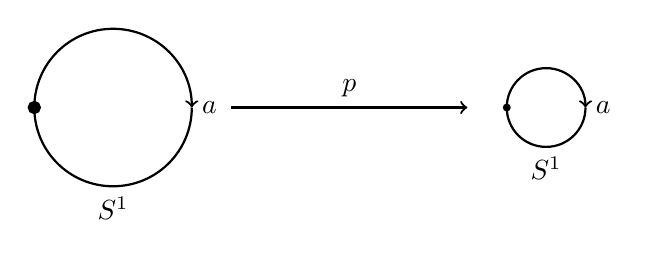
\begin{tikzpicture}[thick]
      \begin{scope}[shift={(3,0)}, scale=0.5]
        \filldraw (0,0) circle (2pt);
\draw [->] (0,0) to [bend left=45] (1,1)  to [bend left=45] (2,0) node [right] {$a$};
\draw (2,0) to [bend left=45] (1,-1)  node [below] {$S^1$} to [bend left=45] (0,0);

      \end{scope}

      \draw [->] (-0.5,0) to node[midway, above] {$p$} (2.5,0);

      \begin{scope}[shift={(-3,0)}]
        \filldraw (0,0) circle (2pt);
\draw [->] (0,0) to [bend left=45] (1,1)  to [bend left=45] (2,0) node [right] {$a$};
\draw (2,0) to [bend left=45] (1,-1)  node [below] {$S^1$} to [bend left=45] (0,0);

      \end{scope}
    \end{tikzpicture}
    \caption{2-covering of a circle}
  \end{figure}
  Further, these covering maps form a poset: $nS^1$ is a cover of $mS^1$ if and only if $m$ divides $n$.
  $S^1$ has an infinite covering given by the real line.

  \begin{figure}[H]
  \centering
    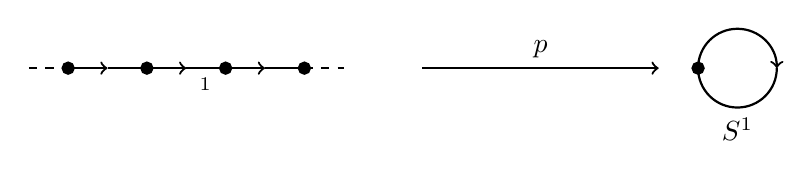
\begin{tikzpicture}[thick]
      \begin{scope}[shift={(3,0)}, scale=0.5]
        \filldraw (0,0) circle (4pt);
        \draw [->] (0,0) to [bend left=45] (1,1) to [bend left=45] (2,0);
        \draw (2,0) to [bend left=45] (1,-1)  node [below] {$S^1$} to [bend left=45] (0,0);
      \end{scope}

      \draw [->] (-0.5,0) to node[midway, above] {$p$} (2.5,0);

      \begin{scope}[shift={(-5,0)}, scale=0.5]
        \filldraw (0,0) circle (4pt)
                  (2,0) circle (4pt)
                  (4,0) circle (4pt)
                  (6,0) circle (4pt);
        \draw [dashed] (-1,0) to (0,0);
        \draw [->] (0,0) to (1,0);
        \draw (1,0) to (2,0);
        \draw [->] (2,0) to (3,0);
        \draw (3,0) to node[midway, below] {$\bbr^1$} (4,0);
        \draw [->] (4,0) to (5,0);
        \draw (5,0) to (6,0);
        \draw [dashed] (6,0) to (7,0);
      \end{scope}
    \end{tikzpicture}
    \caption{Covering of $S^1$ by $\bbr^1$.}
  \end{figure}

  We will show that these covering spaces correspond to the subgroups of $\bbz$ and the inclusions of subgroups correspond to covering maps.
  \begin{align*}
    n \bbz &\longleftrightarrow nS^1 \\
    \set{0} &\longleftrightarrow \bbr^1 \\
    n \bbz \subseteq d \bbz &\longleftrightarrow nS^1 \rightarrow dS^1
  \end{align*}
  This is because the fundamental group of the circle is $\bbz$.


  \subsection{Example: $S^1 \vee S^1$}
  The space $S^1 \vee S^1$ (two circles glued at point) with 1 vertex, 2 edges, and 0 faces has very interesting covering spaces, see Figure \ref{fig:CoveringsOfS1S1}. The meanings of the various notations in Figure \ref{fig:CoveringsOfS1S1} will become clear later.
  \begin{figure}[H]
  \centering
    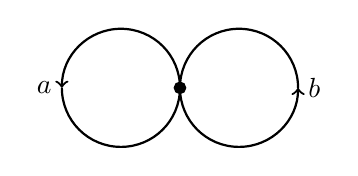
\begin{tikzpicture}[thick, scale=0.75]
      \filldraw (0,0) circle (2.5pt);

\draw [->] (0,0) to [bend right=45] (-1,1) to [bend right=45] (-2,0) node [left] {$a$} ;
\draw (-2,0) to [bend right=45] (-1,-1) to [bend right=45] (0,0);

\draw [->] (0,0) to [bend right=45] (1,-1) to [bend right=45] (2,0) node [right] {$b$};
\draw (2,0) to [bend right=45] (1,1) to [bend right=45] (0,0);

    \end{tikzpicture}
    \caption{$S^1 \vee S^1$}
  \end{figure}

  \begin{figure}[p]
  \centering
    \includegraphics[width=\textwidth]{coveringsOfS1S1.jpg}
    \caption{Coverings of $S^1 \vee S^1$. Image from Algebraic Topology, Allen Hatcher, Chapter 1.}
    \label{fig:CoveringsOfS1S1}
  \end{figure}






  \subsubsection{Example: Gluing diagrams}
  We can form surfaces using 2-complexes, however these are harder to describe on paper.
  Instead, we use a trick called \emph{gluing diagrams}, Figure \ref{fig:GluingDiagrams}.
  These are ways to draw non-planar things on a plane, so there is some ambiguity and gluing going on in a gluing diagram that you should be careful about.

  \begin{qbox}
    In each of the gluing diagrams in Figure \ref{fig:GluingDiagrams}, count the number of vertices, edges, and faces.
  \end{qbox}

  \begin{qbox}
    Show that there are 2-cover maps
    \begin{align*}
      \mbox{Cylinder} &\longrightarrow \mbox{Mobius Strip} \\
      \mbox{Torus} &\longrightarrow \mbox{Klein Bottle} \\
      \mbox{Sphere } S^2 &\longrightarrow \mbox{Real projective space}
    \end{align*}
  \end{qbox}

  \begin{qbox}
    Guess the poset of covers of
    \begin{enumerate}
      \item Cylinder,
      \item Mobius Strip,
      \item Torus.
    \end{enumerate}
    Can you interpret these posets as subgroups of some groups?
  \end{qbox}


  \begin{figure}[p]
    \centering
    \includegraphics[width=0.8\textwidth]{cylinderGluingDiagram.png}
    \includegraphics[width=0.8\textwidth]{MobiusStripGluingDiagram.png}

    \includegraphics[width=0.8\textwidth]{torusGluingDiagram.png}
    \includegraphics[width=0.8\textwidth]{KleinBottleGluingDiagram.png}

    \includegraphics[width=0.8\textwidth]{RP2GluingDiagram.png}
    \caption{Gluing diagrams for cylinder, Mobius strip, torus, Klein bottle, real projective space respectively. Images from BMC Notes on Surfaces by Maia Averett.}
    \label{fig:GluingDiagrams}
  \end{figure}
